% !LW recipe = pdflatex (quick build)
\documentclass[tikz,border=3pt]{standalone}
\usepackage{tikz}
\usetikzlibrary{calc}

\begin{document}

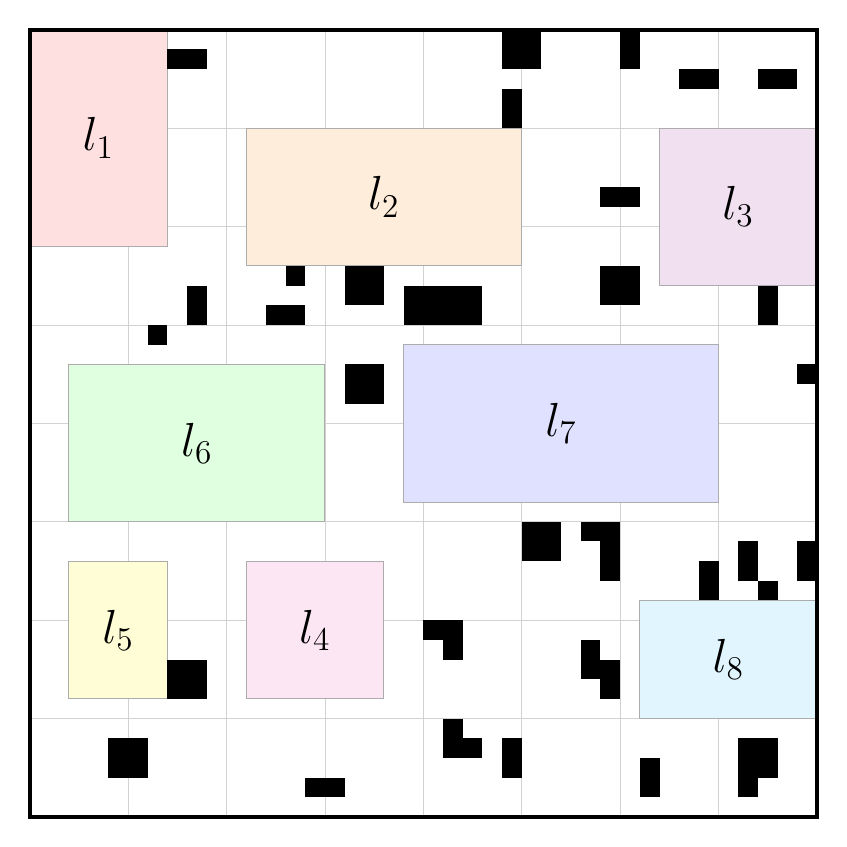
\begin{tikzpicture}[x=0.25cm,y=0.25cm]

% ------------------------------------------------------------------
% Editable parameters
% Each region is specified as: \region{label}{x}{y}{width}{height}{fill}
% Change x, y, width, and height to move or resize a region.
% The workspace is a 40-by-40 square.
% ------------------------------------------------------------------
\newcommand{\region}[6]{%
  \filldraw[fill=#6, draw=gray!65, line width=0.35pt]
    (#2,#3) rectangle ++(#4,#5);
  \node[font=\fontfamily{ptm}\fontsize{17}{19}\selectfont\itshape]
    at ($(#2,#3)+(#4/2,#5/2)$) {$l_{#1}$};
}

% Obstacles are specified as: \obstacle{x}{y}{width}{height}
% Their coordinates and sizes can also be edited independently.
\newcommand{\obstacle}[4]{%
  \fill[black] (#1,#2) rectangle ++(#3,#4);
}

% Major grid lines every 5 units.
\foreach \v in {0,5,...,40}{
  \draw[gray!35, line width=0.25pt] (\v,0) -- (\v,40);
  \draw[gray!35, line width=0.25pt] (0,\v) -- (40,\v);
}

% Regions: edit only the four geometric parameters when needed.
\region{1}{0}{29}{7}{11}{red!12}
\region{2}{11}{28}{14}{7}{orange!14}
\region{3}{32}{27}{8}{8}{violet!12}
\region{4}{11}{6}{7}{7}{magenta!10}
\region{5}{2}{6}{5}{7}{yellow!16}
\region{6}{2}{15}{13}{8}{green!12}
\region{7}{19}{16}{16}{8}{blue!12}
\region{8}{31}{5}{9}{6}{cyan!12}

% Obstacles inherited from the workspace map.
\obstacle{7}{38}{2}{1}
\obstacle{24}{38}{2}{2}
\obstacle{30}{38}{1}{2}
\obstacle{33}{37}{2}{1}
\obstacle{37}{37}{2}{1}
\obstacle{24}{35}{1}{2}
\obstacle{29}{31}{2}{1}
\obstacle{20}{25}{1}{2}
\obstacle{13}{27}{1}{1}
\obstacle{16}{26}{2}{2}
\obstacle{12}{25}{2}{1}
\obstacle{19}{25}{4}{2}
\obstacle{6}{24}{1}{1}
\obstacle{8}{25}{1}{2}
\obstacle{29}{26}{2}{2}
\obstacle{37}{25}{1}{2}
\obstacle{16}{21}{2}{2}
\obstacle{39}{22}{1}{1}
\obstacle{21}{8}{1}{2}
\obstacle{20}{9}{1}{1}
\obstacle{25}{13}{2}{2}
\obstacle{28}{14}{2}{1}
\obstacle{29}{12}{1}{2}
\obstacle{34}{11}{1}{2}
\obstacle{36}{12}{1}{2}
\obstacle{37}{11}{1}{1}
\obstacle{39}{12}{1}{2}
\obstacle{14}{1}{2}{1}
\obstacle{21}{3}{1}{2}
\obstacle{22}{3}{1}{1}
\obstacle{24}{2}{1}{2}
\obstacle{28}{7}{1}{2}
\obstacle{29}{6}{1}{2}
\obstacle{31}{1}{1}{2}
\obstacle{36}{1}{1}{3}
\obstacle{37}{2}{1}{2}
\obstacle{7}{6}{2}{2}
\obstacle{4}{2}{2}{2}
% Thick black outer frame.
\draw[black, line width=1.4pt] (0,0) rectangle (40,40);

\end{tikzpicture}
\end{document}
